%%%% CS 383 HW #5 - hw5-team_lambda.tex
%%%% Due on BBLearn before 10pm on Friday 3/25/2016


%##########################################################################################################################################################################
% Header
%##########################################################################################################################################################################
\documentclass[11pt]{report}

\usepackage{graphicx}
\usepackage{caption}

\marginparwidth 0.5in 
\oddsidemargin 0.25in 
\evensidemargin 0.25in 
\marginparsep 0.25in
\topmargin 0.0in 
\textwidth 6in \textheight 8.5in

\title{Squire: A Collaborative Software Development Tool}
\author{jank6275, mora5651, boss2849, bolt1003, gall7417, brec9824, snev7821, mars2681}

\begin{document}

\maketitle

\tableofcontents


%##########################################################################################################################################################################
% Overview
%##########################################################################################################################################################################
\chapter{Overview and Scope}
    \begin{minipage}{1\textwidth}
        \begin{center}
            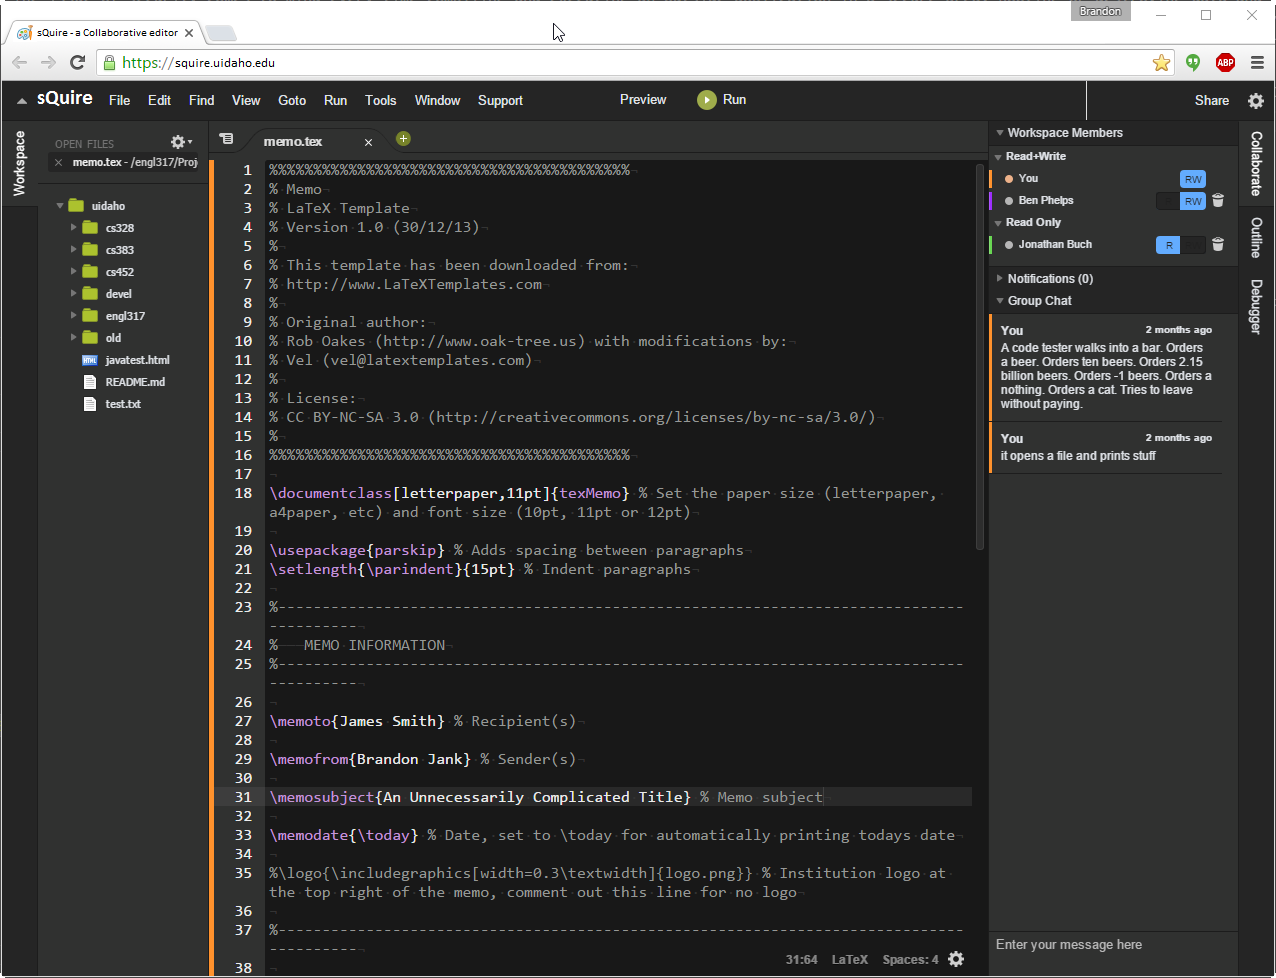
\includegraphics[width=0.7\textwidth]{mockups/mockup-editor-jank6275}
        \end{center}
        \captionof{figure}{"Squire is a web-based collaborative software development environment with a project development center. Squire will allow multiple users to edit files and communicate in real time. Projects can be ``stubbed'' out by a user and then other users can join and/or vote to support for their favorite projects. After a certain amount of support, planning, and documentation is reached for a project, the project becomes a fully fleged project and then community development can start. Think ``kickstarter for code'' where people pledge their help with the project and not just financial support."}
    \end{minipage}


%##########################################################################################################################################################################
% Statecharts
%##########################################################################################################################################################################
\chapter{State Charts}
    \section{Project Forum (snev7821)}
        \begin{minipage}{1\textwidth}
            \begin{center}
                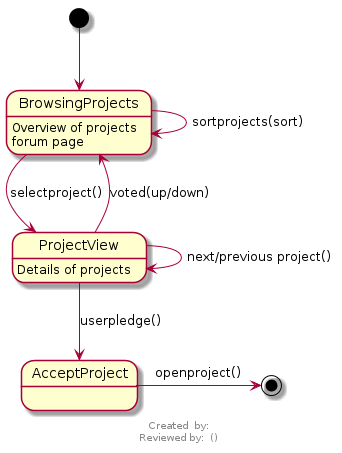
\includegraphics[width=0.5\textwidth]{diagrams/statechart-projectforum}
            \end{center}
            \captionof{figure}{Statechart showing the flow of a user browsing the project forum page}
        \end{minipage}
    
    \section{Settings/Preferences (gall7417)}
        \begin{minipage}{1\textwidth}
            \begin{center}
    %            \includegraphics[width=0.5\textwidth]{diagrams/statechart-settings}
            \end{center}
            \captionof{figure}{Statechart showing the flow of a user changing a user setting}
        \end{minipage}
    
    \section{Compile (boss2849)}
        \begin{minipage}{1\textwidth}
            \begin{center}
                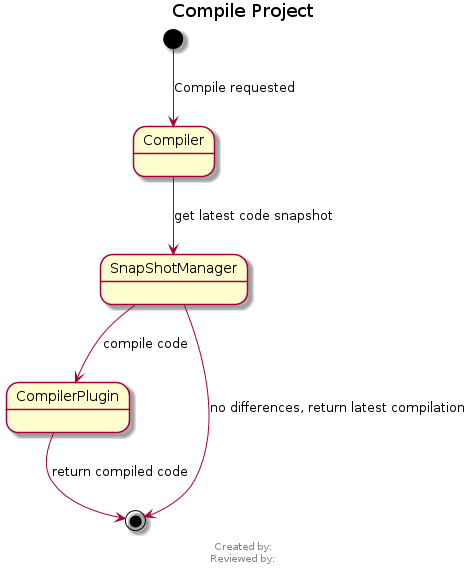
\includegraphics[width=0.5\textwidth]{diagrams/statechart-compile}
            \end{center}
            \captionof{figure}{Statechart showing the flow of a user compiling a file, or entire project.}
        \end{minipage}
        
    \section{Project Management (bolt1003)}
        \begin{minipage}{1\textwidth}
            \begin{center}
                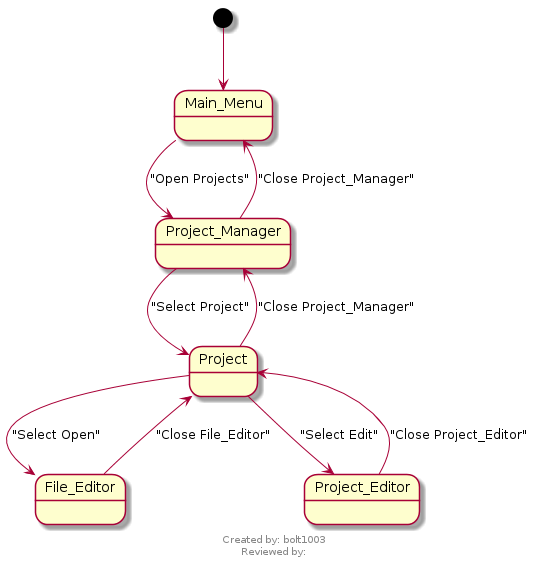
\includegraphics[width=0.5\textwidth]{diagrams/statechart-project_management}
            \end{center}
            \captionof{figure}{.}
        \end{minipage}
        
    \section{Communication (jank6275)}
        \begin{minipage}{1\textwidth}
            \begin{center}
                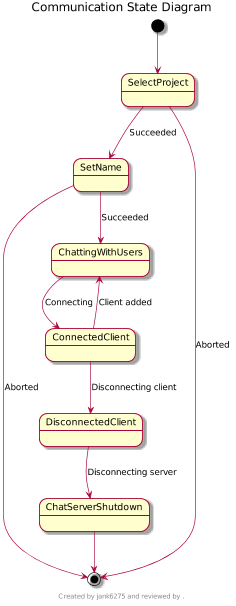
\includegraphics[width=0.5\textwidth]{diagrams/statechart-communication}
            \end{center}
            \captionof{figure}{A statechart that shows the various states of the communication system.}
        \end{minipage}
        
    \section{Authentication (brec9824)}
        \begin{minipage}{1\textwidth}
            \begin{center}
                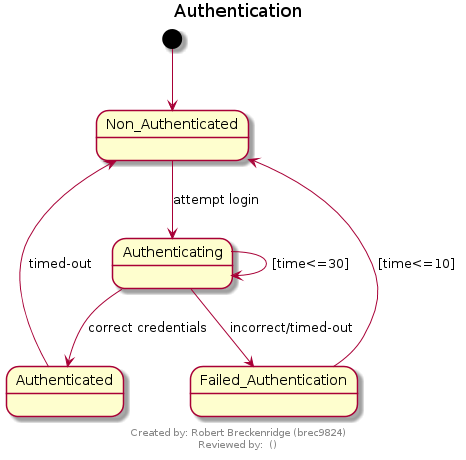
\includegraphics[width=0.5\textwidth]{diagrams/statechart-authentication-brec9824}
            \end{center}
            \captionof{figure}{Statechart showing the flow between states for authentication.}
        \end{minipage}


%##########################################################################################################################################################################
% Mockups
%##########################################################################################################################################################################
\chapter{User Interface Mockups}
    \section{Project Management (bolt1003)}
    \begin{minipage}{1\textwidth}
        \begin{center}
            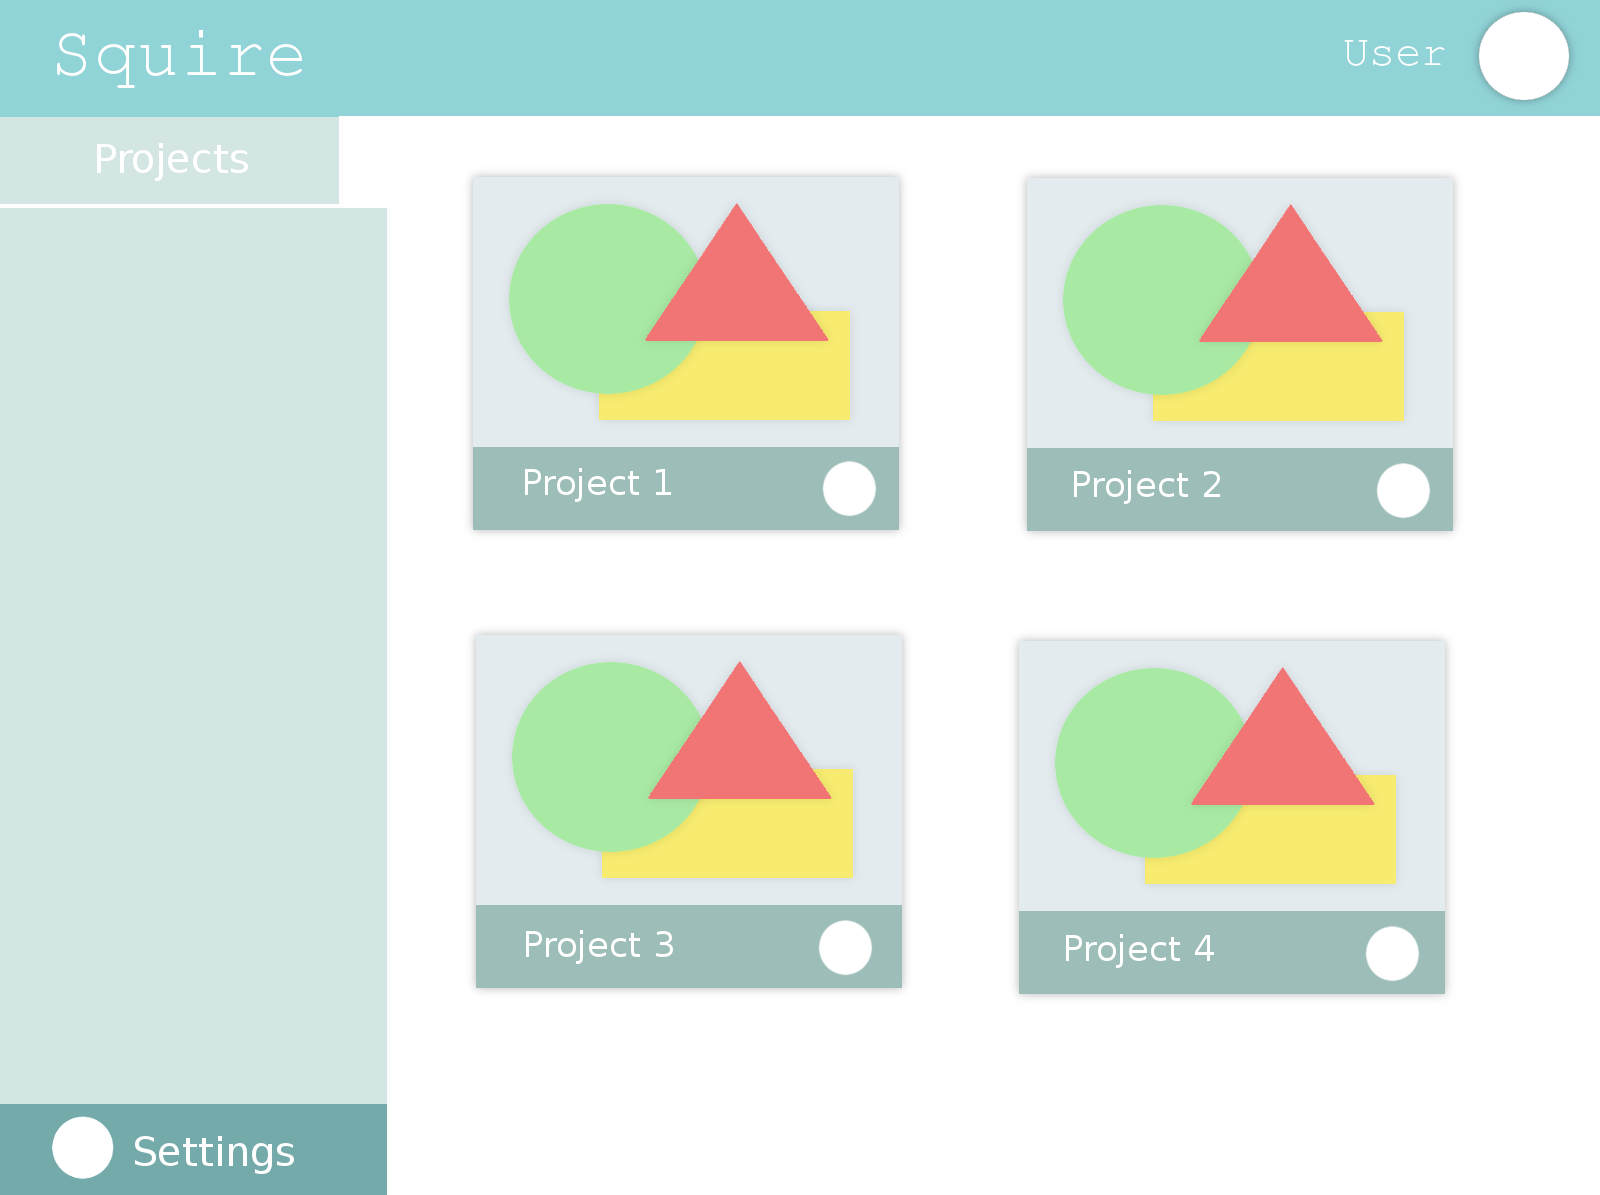
\includegraphics[width=0.9\textwidth]{mockups/mockup-project_management-bolt1003}
        \end{center}
        \captionof{figure}{A possible look for the project management page}
    \end{minipage}
    
    \section{Settings and Preferences (gall7417)}
    \begin{minipage}{1\textwidth}
        \begin{center}
            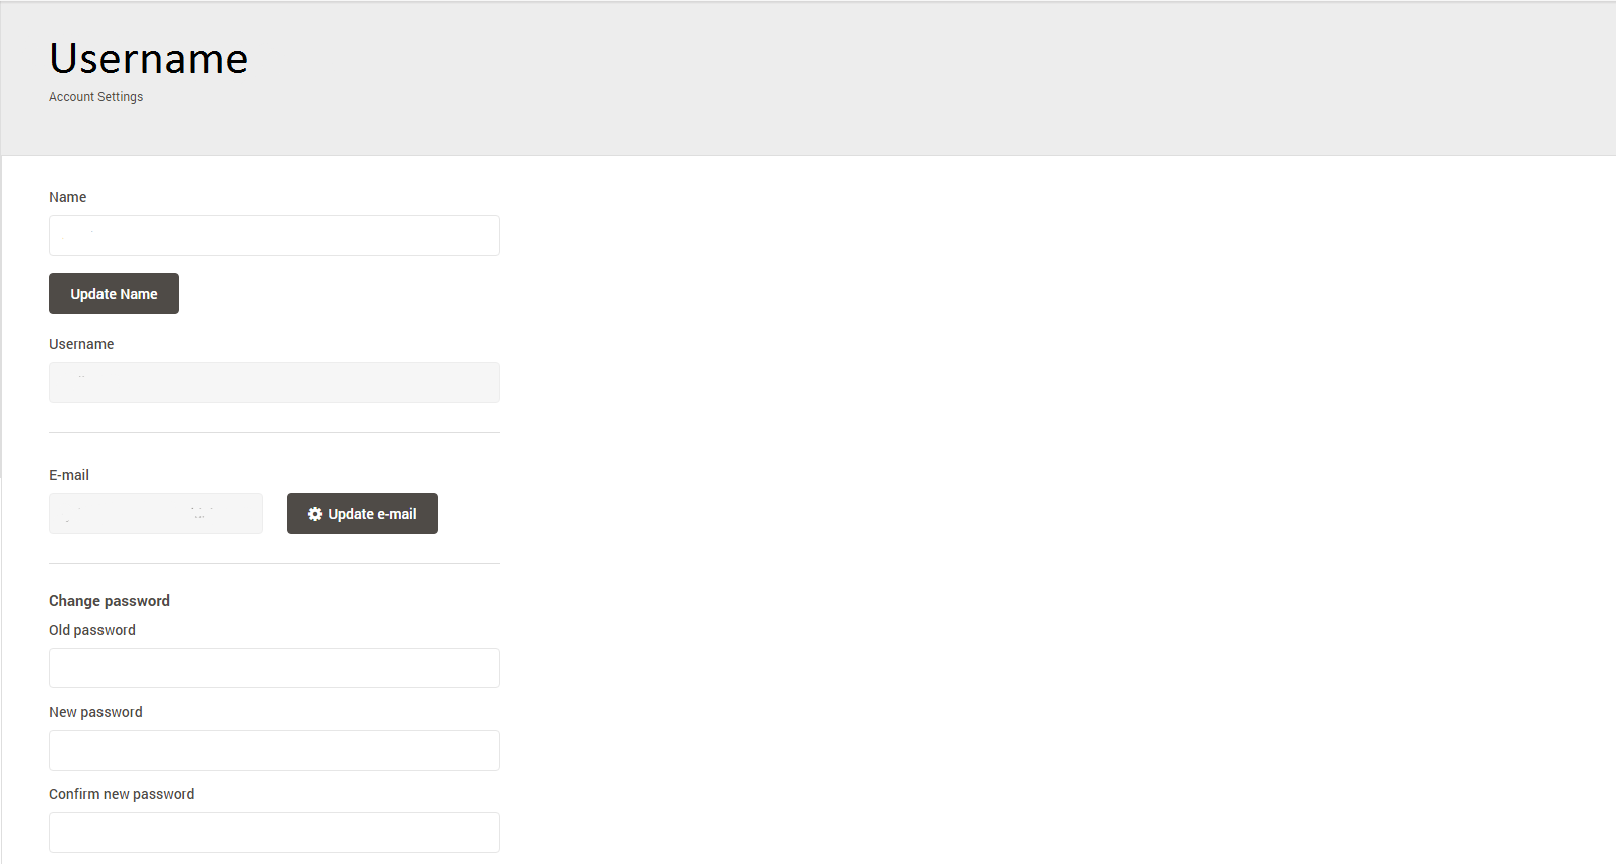
\includegraphics[width=0.9\textwidth]{mockups/mockup-settings-gall7417}
        \end{center}
        \captionof{figure}{Po}
    \end{minipage}
    
    \section{Squire Editor (jank6275)}
    \begin{minipage}{1\textwidth}
        \begin{center}
            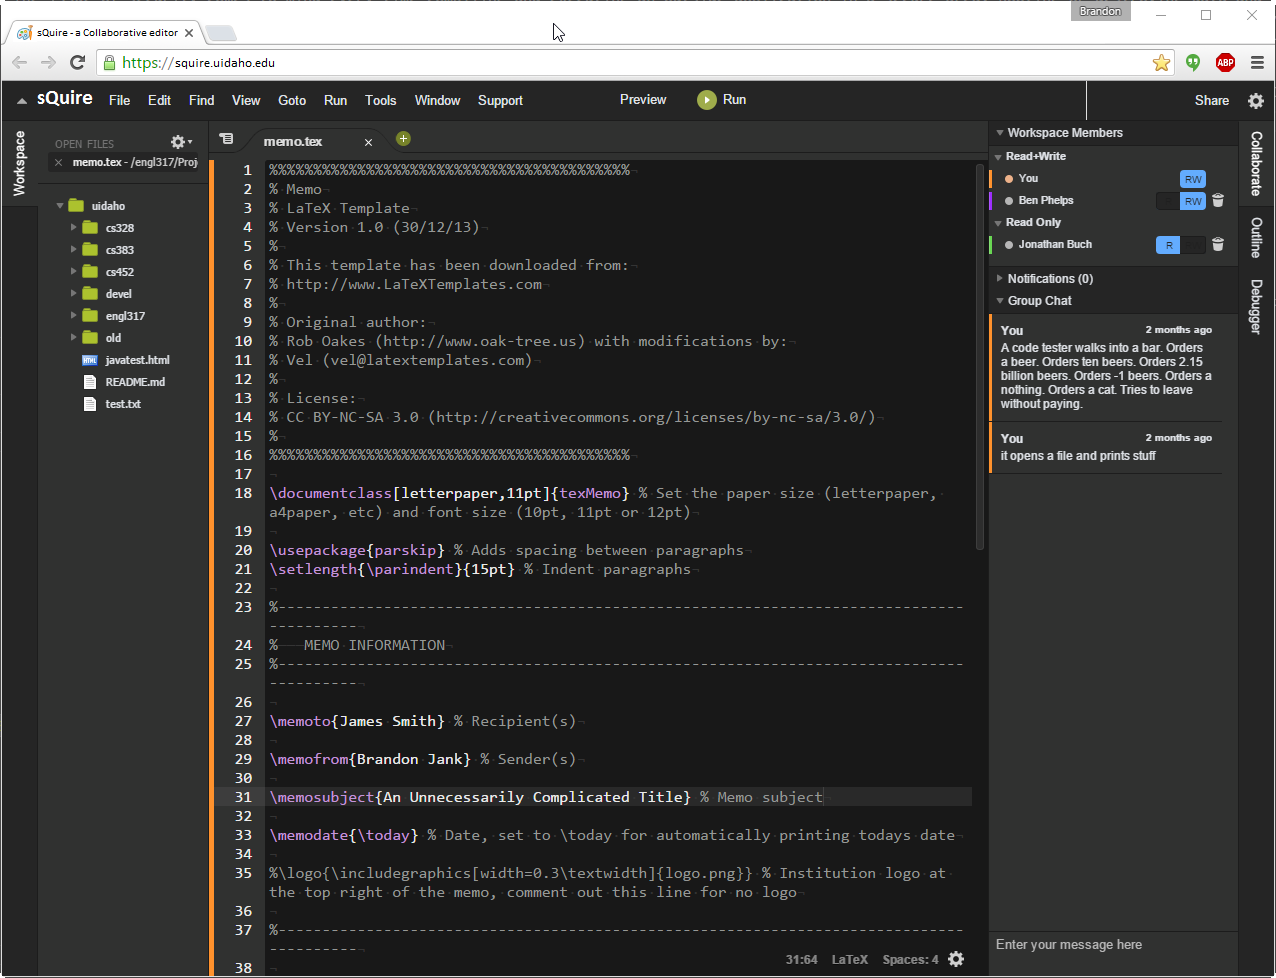
\includegraphics[width=0.9\textwidth]{mockups/mockup-editor-jank6275}
        \end{center}
        \captionof{figure}{What we envision Squire IDE to look like.}
    \end{minipage}
    
    \section{Squire Chat (jank6275)}
    \begin{minipage}{1\textwidth}
        \begin{center}
            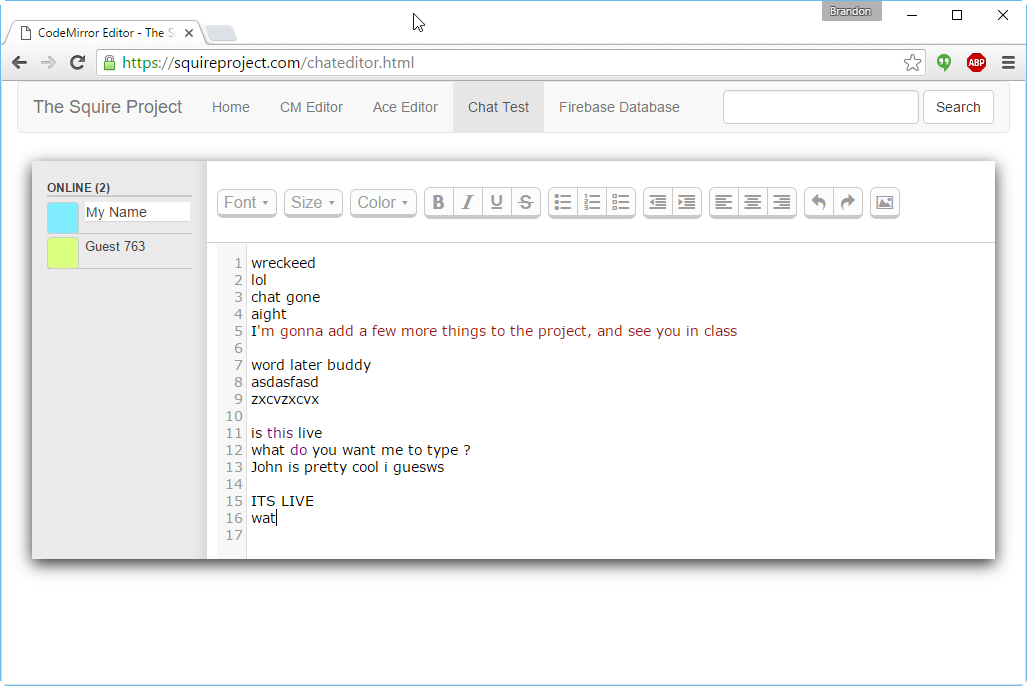
\includegraphics[width=0.9\textwidth]{mockups/mockup-communication-jank6275}
        \end{center}
        \captionof{figure}{How communication could work in squire.}
    \end{minipage}
    
    \section{Project Browser (snev7821)}
    \begin{minipage}{1\textwidth}
        \begin{center}
            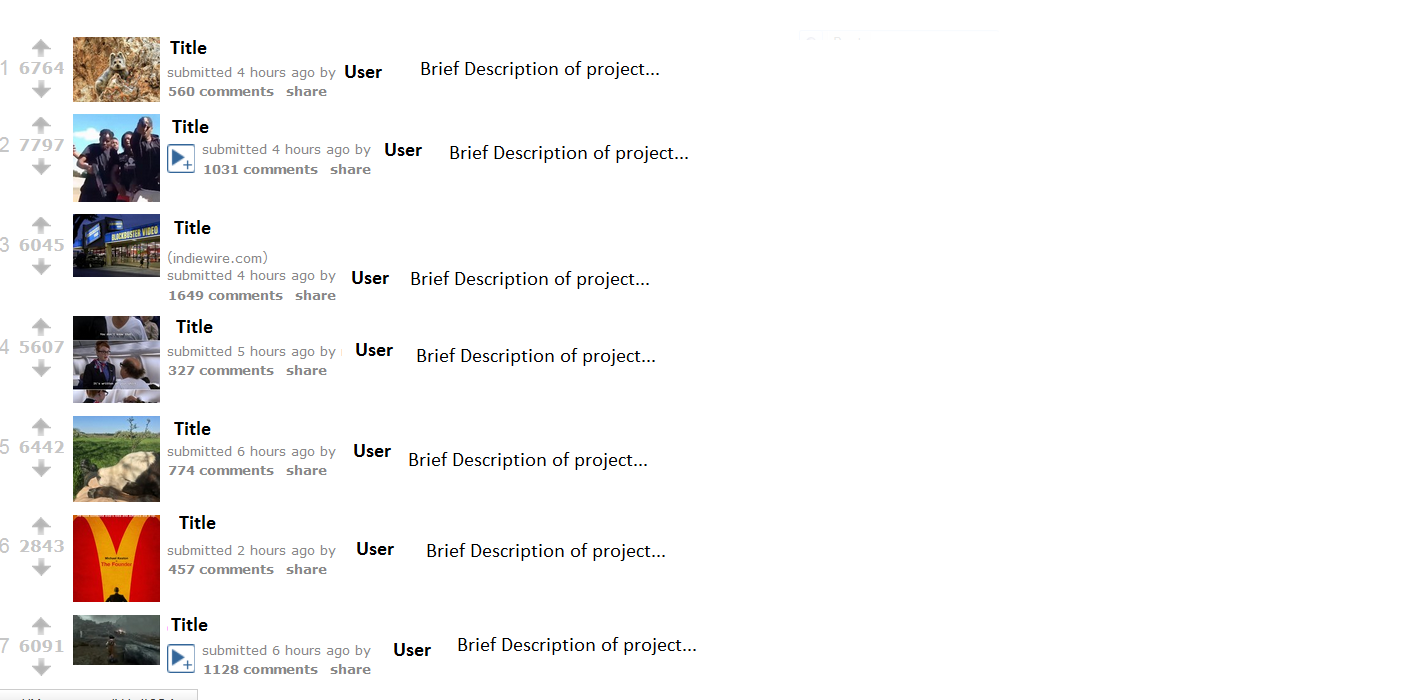
\includegraphics[width=0.9\textwidth]{mockups/mockup-project_browser-snev7821}
        \end{center}
        \captionof{figure}{Created from Paint and Reddit, the project browser may end up looking somewhat similar}
    \end{minipage}
    
    \section{Compile Mockup (boss2849)}
    \begin{minipage}{1\textwidth}
        \begin{center}
            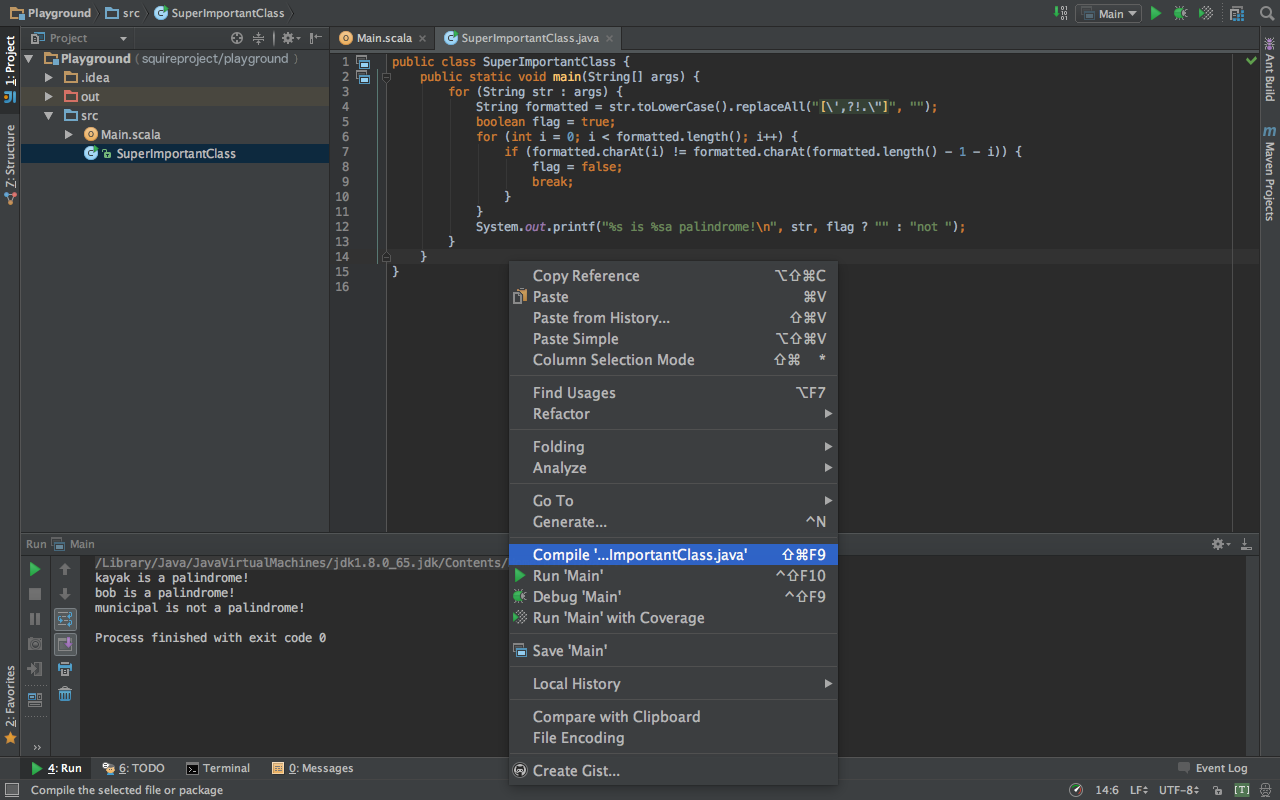
\includegraphics[width=0.9\textwidth]{mockups/mockup-compile-boss2849}
        \end{center}
        \captionof{figure}{A mockup, based off IntelliJ of compiling a file.}
    \end{minipage}

    \section{Syntax Mockup (mars2681)}
    \begin{minipage}{1\textwidth}
        \begin{center}
            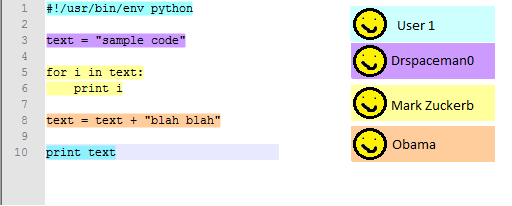
\includegraphics[width=0.9\textwidth]{mockups/mockup-syntax-mars2681}
        \end{center}
        \captionof{figure}{A mockup, created from Notepad++ and paint. Each user's input has its own shade. The light blue shade on Line 10 shows current user's cursor position.}
    \end{minipage}
    
    \section{Home (brec9824)}
    \begin{minipage}{1\textwidth}
        \begin{center}
            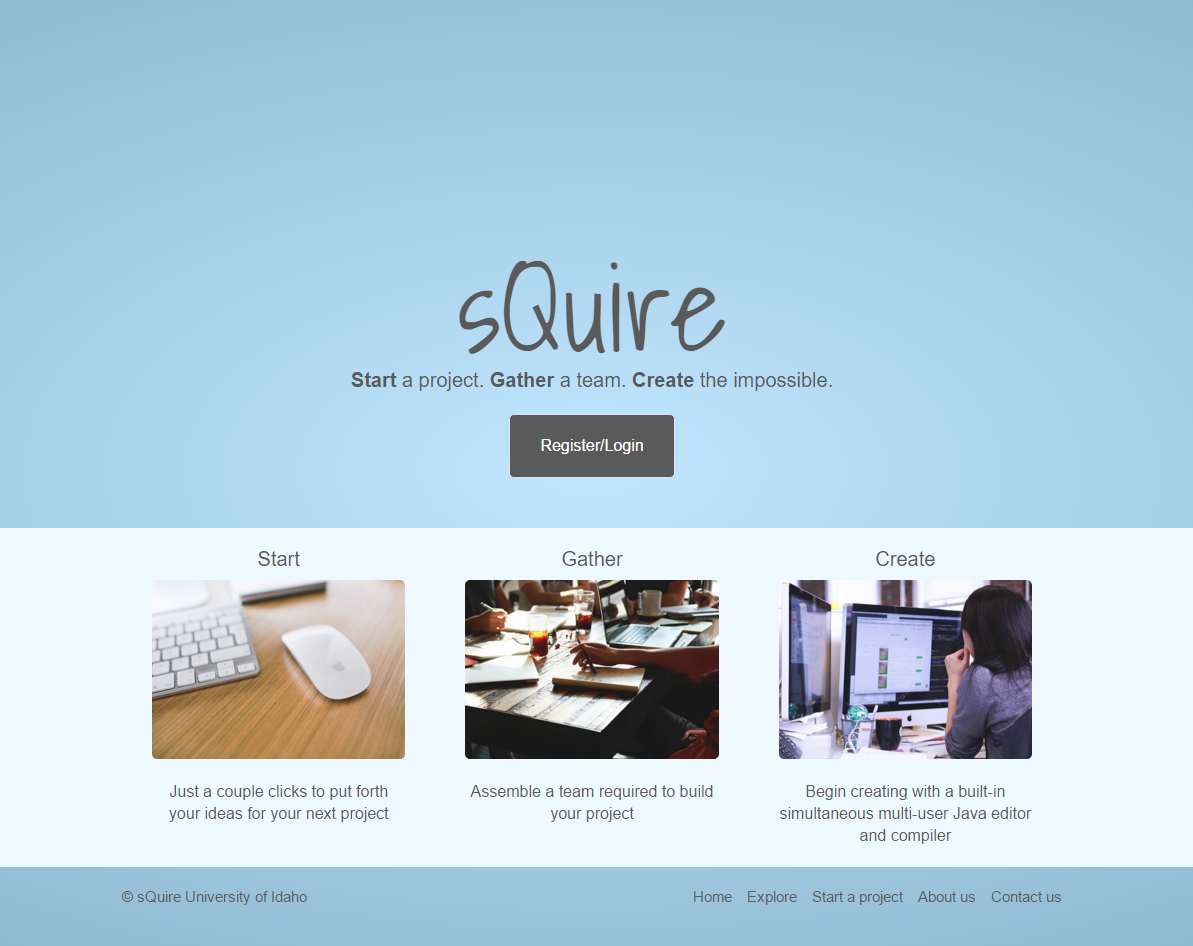
\includegraphics[width=0.9\textwidth]{mockups/mockup-home-brec9824}
        \end{center}
        \captionof{figure}{A mockup for the look of squire's home page. Created using html and css.}
    \end{minipage}
    
    \section{Register (brec9824)}
    \begin{minipage}{1\textwidth}
        \begin{center}
            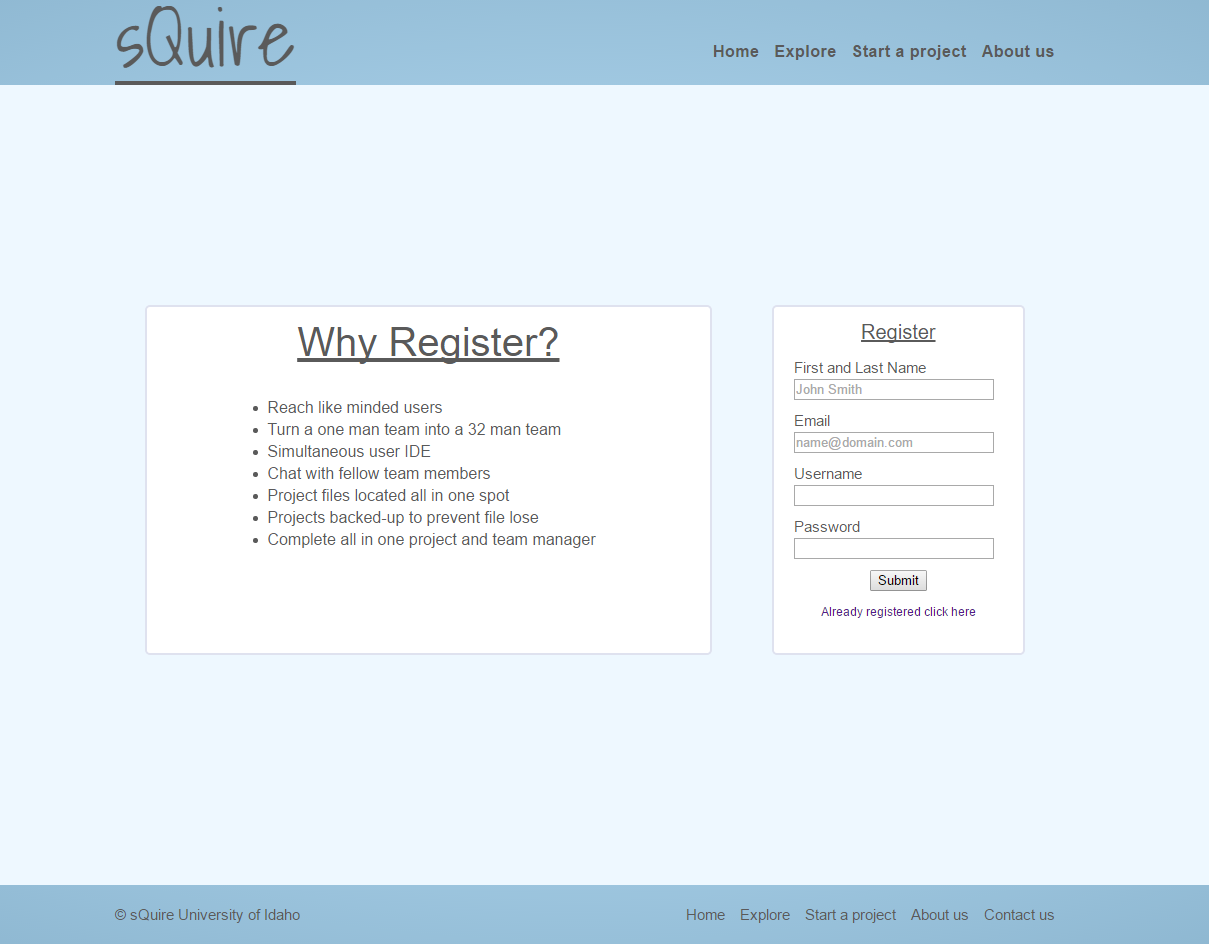
\includegraphics[width=0.9\textwidth]{mockups/mockup-register-brec9824}
        \end{center}
        \captionof{figure}{A mockup for the look of squire's register page. Created using html and css.}
    \end{minipage}
    
     \section{Login (brec9824)}
    \begin{minipage}{1\textwidth}
        \begin{center}
            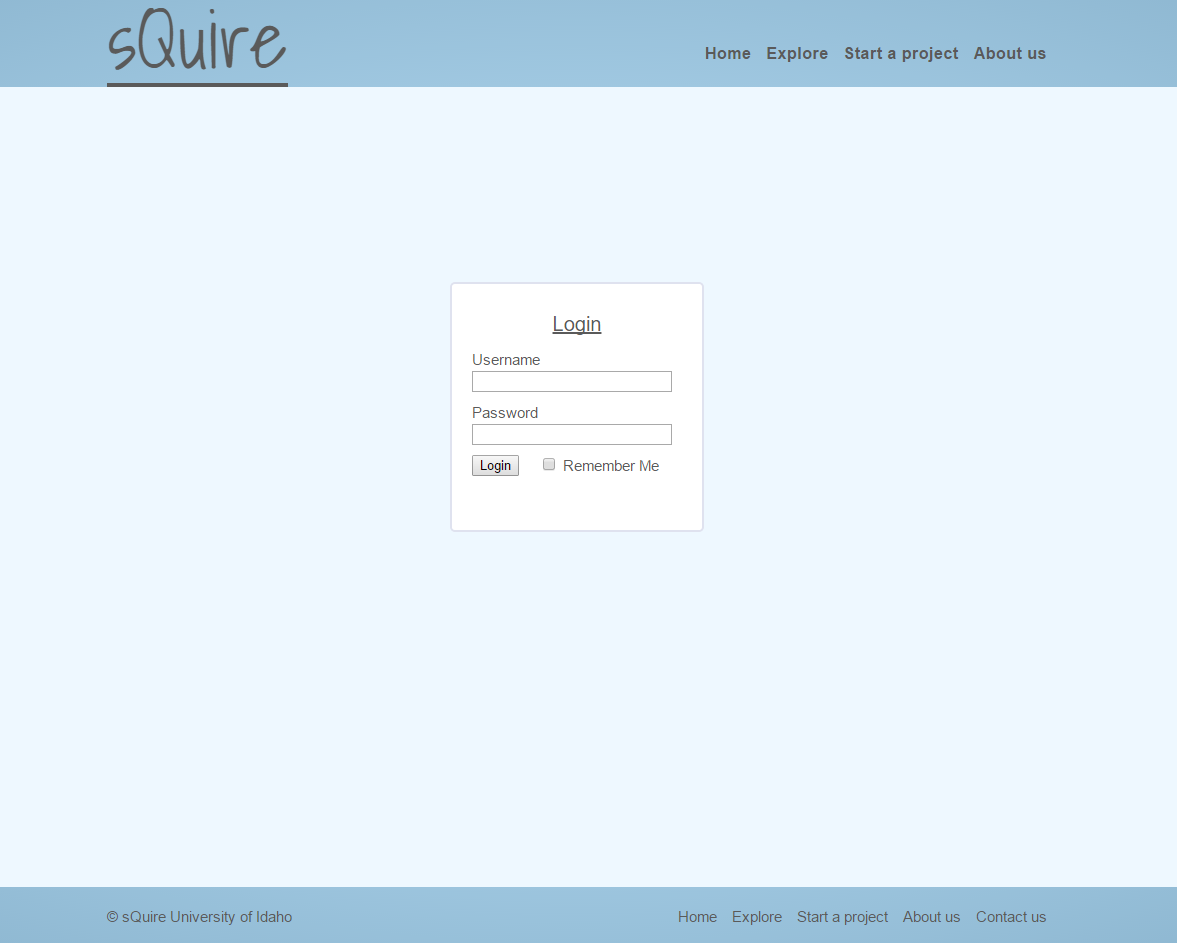
\includegraphics[width=0.9\textwidth]{mockups/mockup-login-brec9824}
        \end{center}
        \captionof{figure}{A mockup for the look of squire's login page. Created using html and css.}
    \end{minipage}
    
    \section{Project Finder (brec9824)}
    \begin{minipage}{1\textwidth}
        \begin{center}
            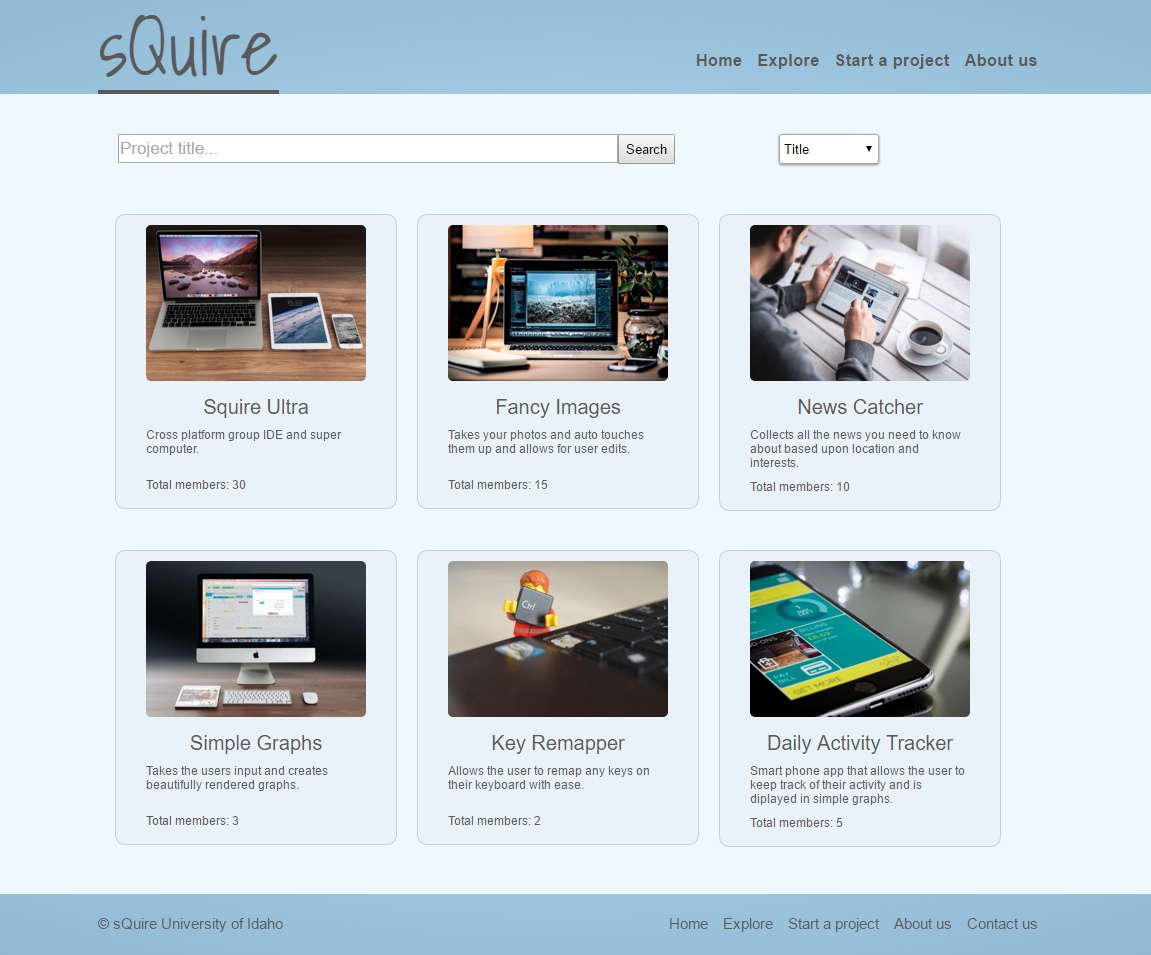
\includegraphics[width=0.9\textwidth]{mockups/mockup-projectfinder-brec9824}
        \end{center}
        \captionof{figure}{A mockup for the look of squire's project finder page. Created using html and css.}
    \end{minipage}
    
    \section{Project Idea (mora5651)}
    \begin{minipage}{1\textwidth}
        \begin{center}
            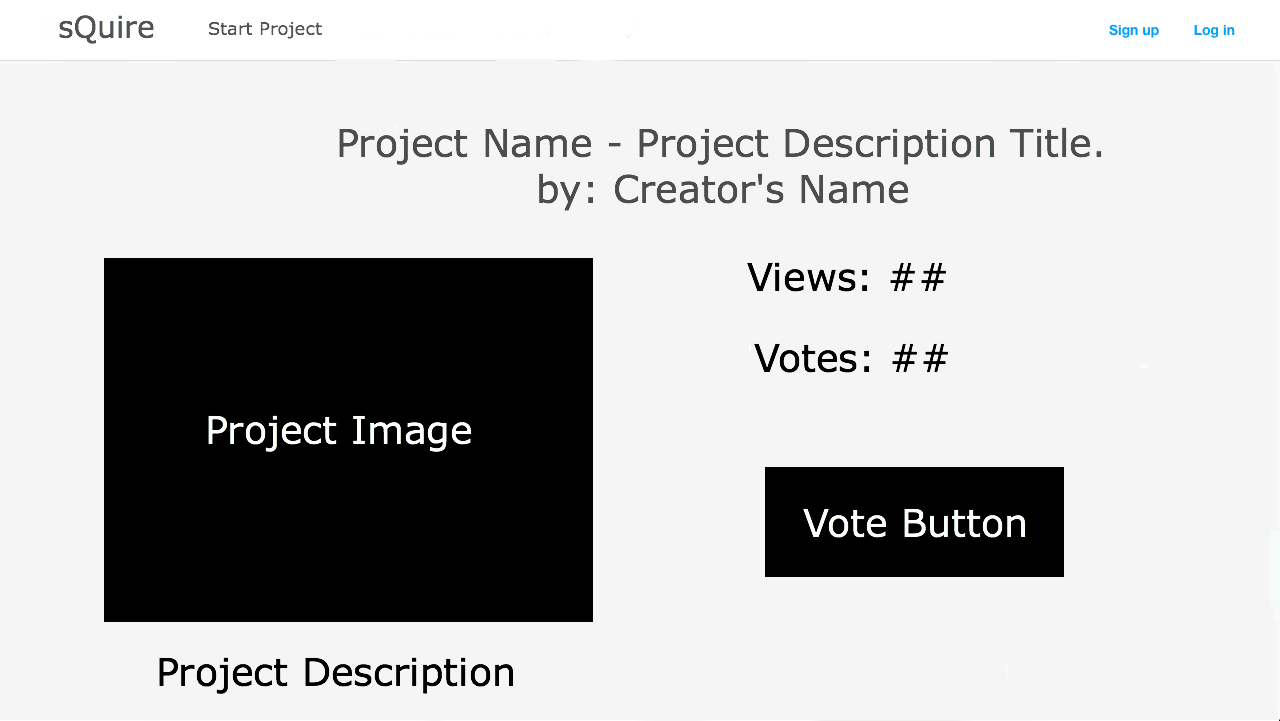
\includegraphics[width=0.9\textwidth]{mockups/mockup-ProjectIdea-mora5651}
        \end{center}
        \captionof{figure}{A mockup of how the project idea page should look like.}
    \end{minipage}

%##########################################################################################################################################################################
% Prototype Implimentations
%##########################################################################################################################################################################
\chapter{Prototype Implementations}
    \section{Server Stack (jank6275)}
    \begin{minipage}{1\textwidth}
        \begin{center}
            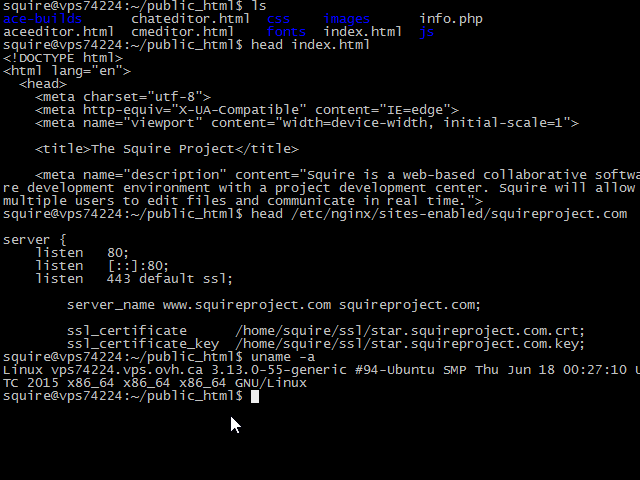
\includegraphics[width=0.9\textwidth]{protos/proto-serverstack-jank6275}
        \end{center}
        \captionof{figure}{The internet domain squireproject.com was registered and an SSL certificate was generated for secure communications. A virtual private server was provisioned and Ubuntu 14.04 installed and then hardened to common network attack vectors. Nginx and MySQL were installed and configured. The web content was written in HTML and bootstrap CSS.}
    \end{minipage}

% EOD
\end{document}